\section{Processi di Supporto}\label{ProcessiSupporto}

\subsection{Documentazione}\label{ProcessiSupporto_Documentazione}

\subsubsection{Descrizione}
Questo capitolo descrive i dettagli su come deve essere redatta e verificata la documentazione durante il ciclo di vita del software. Le norme sono tassativamente valide per tutti i documenti formali.
\subsubsection{Ciclo di Vita della Documentazione}
Il ciclo di vita previsto della documentazione si può suddividere principalmente in tre processi:
\begin{itemize}
	\item \textbf{Sviluppo}: è il processo di stesura, eseguita dal redattore, dove sviluppa il task\glossario assegnato dal \textit{Responsabile}. Una volta terminata la fase di scrittura del documento, il redattore lo segnalerà al \textit{Responsabile}, il quale assegnerà ad un \textit{Verificatore} il compito di analizzare il lavoro svolto;
 	\item \textbf{Verifica}: è il processo eseguito dai \textit{Verificatori} designati dal responsabile. Il loro compito è quello di controllare che il redattore abbia scritto il documento adottando le regole indicate nel documento \textit{Norme di Progetto v3.0.0} ed in maniera grammaticalmente e strutturalmente corretta;
 	\item \textbf{Approvazione}: è il processo conclusivo, in cui il \textit{Verificatore} ha terminato il suo compito di controllo e comunica al \textit{Responsabile} il termine del lavoro. Il \textit{Responsabile} procederà a confermare il documento ed ad eseguirne il rilascio.
\end{itemize}

\subsubsection{Template}
Il gruppo ha deciso di strutturare un template \LaTeX  per dare uniformità a tutti i documenti. Il template facilita e velocizza la stesura, poiché i redattori devono concentrarsi solo ed esclusivamente sul contenuto e non sul layout.

\subsubsection{Struttura Documenti}\label{ProcessiSupporto_Documentazione_StrutturaDocumenti}
Ogni documento segue una determinata struttura, predefinita e accordata dal gruppo:

\paragraph{Prima Pagina} \-\\
La prima pagina di ogni documento ha la stessa struttura: il logo del gruppo centrato in alto con sotto, sempre centrato, il nome del gruppo ed il capitolato scelto. Appena sotto è posizionato il titolo del documento ed una tabella contenente informazioni relative al documento, ovvero la versione, i nome dei redattori e dei verificatori, lo stato (che può essere "confermato" o "work in progress"), l'utilizzo che avrà nel progetto (interno o esterno) ed i destinatari.

\paragraph{Nomenclatura} \-\\
Le seguenti regole valgono per tutti i documenti eccetto per la lettera di presentazione. La nomenclatura è un aspetto fondamentale che abbiamo deciso di strutturare nel seguente modo:
\begin{itemize}
	\item \textbf{vX.Y.Z }: rappresenta la versione del documento con X, Y e Z numeri non negativi:
	\begin{itemize}
		\item \textbf{X}: rapp resenta il numero di pubblicazioni ufficiali del documento in passato; se il valore è 0 significa che il documento non è mai stato pubblicato. Ogni qualvolta viene pubblicato Y e Z vengono azzerati e X viene incrementato di una unità;
		\item \textbf{Y}: identifica il numero di verifiche avvenute con successo, ogni qualvolta viene effettuata una verifica il valore di Z viene azzerato;
		\item \textbf{Z}: identifica il numero di volte che il documento è stato modificato prima di una pubblicazione e/o verifica.
	\end{itemize}
	\item Il formato dei file è \textit{.tex} durante la fase di sviluppo. Dopo l'approvazione da parte del responsabile, verrà creato un file con formato \textit{.pdf} che rappresenta la pubblicazione ufficiale.
\end{itemize}

\paragraph{Struttura Indice} \-\\
In tutta la documentazione, fatta eccezione per i verbali, dopo la pagina di presentazione è presente l'indice del documento. La struttura è standard: numero e titolo del capitolo, eventuali sottosezioni e paragrafi con indicato a fianco la pagina del contenuto. Ogni titolo è un link alla pagina del contenuto.

\paragraph{Struttura Tabelle} \-\\
Il gruppo ha deciso di standardizzare il formato delle tabelle come descritto:
\begin{itemize}
	\item Intestazione a sfondo blu e scritte bianche;
	\item Corpo con righe alternate di colore bianco e grigio, per facilitare la lettura.
\end{itemize}

\paragraph{Elenco Tabelle} \-\\
In tutti i documenti è presente un elenco delle tabelle utilizzate, ove presenti. È posizionato appena dopo l'indice.

\paragraph{Elenco Figure} \-\\
In tutti i documenti è presente un elenco delle figure utilizzate, ove presenti. È posizionato appena dopo l'elenco delle tabelle.

\paragraph{Elenco Riferimenti} \-\\
In tutti i documenti, se necessario, è presente un elenco dei riferimenti alle fonti utilizzate per stilare il documento in esame. È posizionato all'inizio del documento, dopo l'elenco delle tabelle e delle figure.

\paragraph{Piè di Pagina} \-\\
Tutte le pagine, escluso il frontespizio, hanno a destra il numero della pagina ed il numero di pagine totali, così rappresentate: Pagina $x$ di $n$.

\paragraph{Registro delle Modifiche} \-\\
Ogni documento, eccezion fatta per verbali e lettera di presentazione, presenta un registro delle modifiche chiamato "Registro delle Modifiche". È strutturato sotto forma di tabella, che contiene in ordine cronologico tutte le modifiche identificabili dalla versione.  Ogni riga contiene la versione del documento, la data, il nome di chi ha effettuato la modifica, con il suo corrispettivo ruolo, ed infine una breve descrizione della modifica effettuata.

%Per adesso i link sono fucsia

\subsubsection{Norme Tipografiche}
\begin{itemize}
	\item \textbf{Glossario}: i termini contenuti nel glossario si possono identificare dal carattere G maiuscolo e corsivo a pedice della parola interessata, per esempio Norme\textsubscript{G};
	\item \textbf{Nome Gruppo}: in qualsiasi documento, quando si fa riferimento al gruppo si è deciso di adottare il seguente font: \texttt{Agents of S.W.E.};
	\item \textbf{Elenchi Puntati}: ogni elemento di un elenco puntato deve essere seguito da un punto e virgola, eccezion fatta per l'ultimo che sarà seguito dal punto. La prima lettera di ogni item dovrà essere maiuscola;
	\item \textbf{Stile testo}:
	\begin{itemize}
		\item \textbf{Corsivo}: è utilizzato per citare tecnologie esterne, per riferimenti a documentazione (es. \textit{Analisi dei Requisiti, Piano di Progetto}, ecc.), estensione dei file (es. \textit{.pdf, .tex}, ecc.) e per identificare i ruoli del progetto (\textit{Responsabile,Analista}, ecc.);
		\item \textbf{Grassetto}: le parole in grassetto identificano il titolo di una sezione, sottosezione, paragrafo e un elemento di un elenco puntato;
		\item \textbf{URI}:	i link esterni sono evidenti per il colore blu.
	\end{itemize}
	\item \textbf{Formati}:
	\begin{itemize}
		\item \textbf{Date}: sono scritte seguendo il formato YYYY-MM-DD, dove YYYY rappresenta l'anno, MM il mese e DD il giorno;
		\item \textbf{Valuta}: si è adottato il formato XXX.YY con Y che denota le cifre decimali, X le cifre intere ed il punto (.) come delimitatore tra decimale e parte intera.
	\end{itemize}
\end{itemize}


\subsubsection{Documenti Correnti}
\label{ProcessiSupporto_Documentazione_DocumentiCorrenti}
Sono descritti brevemente i documenti formali da consegnare:
\begin{itemize}
	\item \textbf{\textit{Analisi dei Requisiti v3.0.0}}: ha un utilizzo prettamente esterno, inoltre ha l'obiettivo di esporre e scomporre i requisiti\glossario del progetto. Contiene i casi d'uso ed i diagrammi di interazione con l'utente. Viene redatto dagli \textit{Analisti} dopo una profonda analisi del capitolato ed eventuali colloqui con la proponente;
	\item \textbf{\textit{Glossario v3.0.0}}: ha un utilizzo prettamente esterno ed ha lo scopo di dare una definizione ai termini più specifici usati nei documenti formali;
	\item \textbf{\textit{Norme di Progetto v3.0.0}}: è utilizzato internamente, ed espone gli standard e le direttive utilizzate dal gruppo per sviluppare il progetto in tutta la sua interezza;
	\item \textbf{\textit{Piano di Progetto v3.0.0}}: ha un utilizzo esterno, ed espone come il gruppo ha deciso di impiegare le risorse di tempo ed umane;
	\item \textbf{\textit{Piano di Qualifica v3.0.0}}: ha un utilizzo esterno, descrive gli standard e gli obiettivi che il gruppo dovrà raggiungere per garantire la qualità di prodotto e processo;
	\item \textbf{\textit{Manuale Utente v1.0.0}}: ha un utilizzo esterno, descrive le funzionalità del prodotto e spiega, in modo intuitivo e preciso, le modalità di utilizzo del plug-in \textit{G\&B};
	\item \textbf{\textit{Manuale Sviluppatore v1.0.0}}: ha un utilizzo esterno, descrive tutte le informazioni necessarie agli sviluppatori che intenderanno estendere o migliorare il plug-in \textit{G\&B}.
\end{itemize}

\subsubsection{Ambiente}\label{ProcessiSupporto_Documentazione_Ambiente}
Per uniformare e strutturare al meglio la scrittura dei documenti il gruppo ha adottato il formato \LaTeX.
\textit{TexMaker} è utilizzato per la stesura, si è optato per questo editor perchè open-source ed integra un controllo ortografico della lingua italiana.
Per la costruzione dei diagrammi è stato optato per l'utilizzo di script in \textit{Python}, scritti e testati dal gruppo, per uniformare la procedura in tutta la documentazione.

\subsection{Qualità} \label{qualita}

\subsubsection{Introduzione}
Il contenuto di questa sezione descrive le metriche e i criteri di qualità di processo e prodotto che vengono utilizzati nel documento \textit{Piano di Qualifica}.

\subsubsection{Classificazione Processi}
Per garantire una corretta struttura, il gruppo ha deciso di introdurre una nomenclatura per identificare i processi descritti nel documento. I processi saranno identificati così:
\begin{center}
	\textbf{PRC[num]}
\end{center}
dove:
\begin{itemize}
	\item \textbf{num}: rappresenta il numero identificativo del processo formato da due cifre intere a partire da 1, unico per tutto il documento.
\end{itemize}

\subsubsection{Classificazione Metriche}
Per garantire una corretta struttura, il gruppo ha deciso di introdurre una nomenclatura per identificare le metriche utilizzate. Si potranno quindi identificare cosi:
\begin{center}
	\textbf{MT[mcat][cat][num]}
\end{center}
\begin{itemize}
		\item \textbf{mcat}: identifica le metriche in base a quale macrocategoria andranno a misurare. Può assumere i seguenti valori:
	\begin{itemize}
		\item \textbf{PC}: per indicare le metriche di processo;
		\item \textbf{PD}: per indicare le metriche di prodotto;
		\item \textbf{TS}: per indicare le metriche di test.
	\end{itemize}
	\item \textbf{cat}: identifica la categoria di appartenenza, se esiste, altrimenti è vuota. Per le metriche di prodotto può assumere i seguenti valori:
	\begin{itemize}
		\item \textbf{D}: per indicare i documenti;
		\item \textbf{S}: per indicare il software.
	\end{itemize}

	\item \textbf{num}: identificativo univoco formato da due cifre intere a partire da 1.
\end{itemize}

\subsubsection{Controllo qualità di processo e metriche} \label{ControlloQualita_Processo}
La qualità di processo è raggiunta tramite l'utilizzo di metodi e modelli che garantiscono il corretto procedimento delle fasi di sviluppo del processo. Il team sfrutta le potenzialità del metodo PDCA, descritto nell'appendice \ref{PDCASection}, ottenendo miglioramenti continui nelle qualità di processo e verifica in modo da avere una maggiore qualità nel prodotto risultante. Inoltre verrà utilizzato lo standard ISO/IEC 15504, comunemente conosciuto con l'acronimo SPICE, che misurerà il livello di maturità dei processi.\-\\
Le seguenti metriche sono utilizzate per la valutazione dell'efficacia e dell'efficienza degli stessi.

\paragraph{MTPC01 Schedule Variance (SV)}\-\\
\'E un indice che consente di rilevare se l'andamento del progetto è in linea con quanto pianificato nella baseline\glossario. Può essere utile al cliente per verificare quantitativamente se il team di sviluppo del progetto è in linea con i tempi. \-\\
Calcolo:\-\\
\begin{center}
	\item \textbf{SV = BCWP - BCWS}
\end{center}
dove:
\begin{itemize}
	\item BCWP: valore delle attività realizzate alla data odierna (in giorni);
	\item BCWS: costo pianificato per realizzare le attività alla data odierna (in giorni).
\end{itemize}
Se SV > 0 significa che il progetto sta producendo con maggiore velocità prevista.

\paragraph{MTPC02 Budget Variance (BV)}\-\\
\'E un indice calcolato che permette di rilevare la differenza tra i costi previsti e quelli reali alla data odierna. \\
Calcolo:
\begin{center}
	\item \textbf{BV = BCWS - ACWP}
\end{center} 
dove:
\begin{itemize}
	\item BCWS: costo pianificato per realizzare le attività alla data odierna (in euro);
	\item ACWP: costo effettivo sostenuto per completare le attività alla data odierna (in euro).
\end{itemize}
Se BV > 0 significa che il progetto sta risparmiando sui costi prestabiliti, se BV = 0 significa che il progetto sta mantenendo i costi prefissati, se BV < 0 significa che il progetto sta superando il budget imposto.

\paragraph{MTPC03 Estimated At Completion (EAC)}\-\\
Indice che rappresenta la stima dei costi mancanti. Viene calcolato man mano che il progetto procede ed è fondamentale per attività di pianificazione. \\
Calcolo:
\begin{center}
	\item \textbf{EAC = ACWP + ETC}
\end{center}
dove:
\begin{itemize}
	\item ACWP: costo effettivo sostenuto per completare le attività alla data odierna (in euro);
	\item ETC: valore stimato per la realizzazione delle attività mancanti (in euro).
\end{itemize}

\iffalse
\paragraph{MTPC04 Cost Variance(CV)}\-\\
Indice che quantifica la produttività o efficienza monitorando se il valore del costo realmente maturato è minore, maggiore o uguale al costo effettivo.
Calcolo:
\begin{center}
	\item \textbf{CV = BCWP - ACWP}
\end{center}
dove:
\begin{itemize}
	\item BCWP: valore delle attività realizzate alla data odierna(in euro o giorni);
	\item ACWP: costo effettivo sostenuto per completare le attività alla data odierna(in euro o giorni).
\end{itemize}
Se CV > 0 significa che il progetto produce con maggior efficienza e minor costo.
\fi

\paragraph{Code Coverage}\-\\
Le operazioni di verifica della qualità sul software vengono eseguite seguendo le metriche principali sotto elencate:
\begin{itemize}
	\item \textbf{MTPC04 Function Coverage}: verificare che una funzione sia chiamata;
	\item \textbf{MTPC05 Statement Coverage}: verificare che ogni statement del codice sia eseguito, e non ci sia quindi codice che non verrà mai preso in considerazione;
	\item \textbf{MTPC06 Branch Coverage}: verificare che tutti i possibili percorsi delle strutture di controllo (del tipo \texttt{if, case}, ecc.) siano stati eseguiti.
	\item \textbf{MTPC07 Condition Coverage}: verificare che ogni condizione booleana sia considerata sia vera che falsa.
\end{itemize}

\paragraph{MTPC08 Rischi non preventivati}\-\\
Indice numerico incrementale a partire da 0. Indica il numero di rischi non preventivati che si verificano e vengono considerati durante la corrente fase del progetto. La misurazione avviene incrementando il valore per ogni rischio (non individuato precedentemente) che viene rilevato, il valore viene azzerato per ogni fase del progetto.

\paragraph{MTTS9 Percentuale di test passati}\-\\
Indica la percentuale di test passati, utile per misurare l'avanzamento qualitativo. La misurazione avviene:
\begin{center}
	\item $PTP = \frac{TP}{TT}*100$
\end{center}
dove PTP è la percentuale finale di test passati, TP sono i test passati e TT i test totali eseguiti.

\paragraph{MTTS10 Percentuale di test falliti}\-\\
Indica la percentuale di test falliti. La misurazione avviene:
\begin{center}
	\item $PTF = \frac{TF}{TT}*100$
\end{center}
dove PTF è la percentuale finale di test falliti, TF sono i test passati e TT i test totali eseguiti.

\paragraph{MTTS11 Percentuale di difetti sistemati}\-\\
Indica la percentuale di bug/difetti sistemati, indice utile per misurare l'avanzamento. La misurazione avviene:
\begin{center}
	\item $PDS = \frac{DS}{DT}*100$
\end{center}
dove PDS è la percentuale calcolata, DS i difetti sistemati e DT i difetti totali.

\paragraph{MTTS12 Tempo medio di risoluzione degli errori}\-\\
Indice calcolato sul tempo medio della risoluzione di bug creati dal team durante lo sviluppo. Utile per considerare abilità e tempo di assorbimento di un bug nel sistema. La misurazione avviene:
\begin{center}
	\item $TMRE = \frac{TRE}{NE}$
\end{center}
dove TMRE è il tempo medio calcolato, TRE il tempo totale per la risoluzione degli errori e NE il numero degli errori.

\paragraph{MTTS13 Numero medio di bug trovati per test}\-\\
Indica il numero medio di bug trovati eseguendo i test. \'E un indice utile per verificare la qualità dei test e del sistema in generale. La misurazione avviene:
\begin{center}
	\item $MBT = \frac{NB}{NT}$
\end{center}
dove MBT è la media calcolata, NB il numero di bug rilevati e NT il numero dei test.

\iffalse 
\paragraph{MTTS14 Difetti trovati per requisito}\-\\
Indice numerico che rappresenta il numero medio di test eseguiti per requisito. Utile per verificare che il sistema soddisfi i requisiti a pieno. La misurazione avviene:
\begin{center}
	\item $MDR = \frac{TDR}{TR}$
\end{center}
dove MDR è la media calcolata, TDR il numero totale di difetti trovati e TR il numero totale di requisiti.
\fi

\subsubsection{Metriche per la qualità di prodotto}
Le seguenti metriche sono utilizzate per misurare qualitativamente il prodotto.

\iffalse
\paragraph{MTTS15 Numero di test eseguiti per requisito}\-\\
\fi

\paragraph{MTPDD14 Indice di Gulpease}\-\\
Il gruppo ha deciso di utilizzare l'\textit{indice di Gulpease}\glossario\footnote{\url{https://it.wikipedia.org/wiki/Indice\_Gulpease}} per misurare la leggibilità di un testo. \'E stato sviluppato appositamente uno script in \textit{Python} per automatizzare la procedura e allo stesso modo velocizzarla. La procedura verrà utilizzata a documento terminato e completo così da valutare il lavoro svolto dai redattori.

\paragraph{MTPDD15 Correttezza Ortografica}\-\\
La correttezza ortografica è un aspetto importante che non accetta errori, i documenti al momento della pubblicazione sono corretti. Verranno utilizzati appositi strumenti che supporteranno la correzione. Il software \textit{TexMaker}, per esempio, integra un segnalatore automatico degli errori grammaticali. 

\paragraph{MTPDS16 Soddisfacimento Requisiti Obbligatori}\-\\
Indicatore percentuale che verifica che tutti i requisiti obbligatori siano soddisfatti. Condizione necessaria al fine di rispettare il contratto. La misurazione avviene:
\begin{center}
	\item $PRO = \frac{ROS}{ROT}*100$
\end{center}
dove PRO è la percentuale di requisiti obbligatori soddisfatti, ROS i requisiti obbligatori soddisfatti e ROT i requisiti obbligatori totali.

\paragraph{MTPDS17 Soddisfacimento Requisiti Opzionali Scelti}\-\\
Indicatore percentuale che verifica se tutti i requisiti opzionali scelti siano soddisfatti. Condizione necessaria al fine di rispettare il contratto. La misurazione avviene:
\begin{center}
	\item $PRP = \frac{RPS}{RPT}*100$
\end{center}
dove PRP è la percentuale di requisiti opzionali scelti soddisfatti, RPS i requisiti opzionali scelti soddisfatti e RPT i requisiti opzionali scelti totali.

\paragraph{MTPDS18 Tempo Medio di Comprensione}\-\\
Indica il tempo medio che l'utente impiega per comprendere cosa può svolgere il sistema. \'E misurato in minuti ed è rilevato attraverso test a persone esterne al team di sviluppo.

\paragraph{MTPDS19 Tempo Medio di Apprendimento}\-\\
Indica il tempo medio che l'utente impiega per riuscire a utilizzare a pieno il software e tutte le sue funzionalità. \'E misurato in minuti ed è rilevato tramite test a persone esterne al team di sviluppo. 

\iffalse
\paragraph{MTPDS25 Percentuale Commenti/Codice}\-\\
Indica le righe di commenti presente rispetto al codice. \'E calcolato per ogni procedura e non per l'intera codebase. La misurazione avviene:
\begin{center}
	\item $PC = \frac{RC}{RT}*100$
\end{center}
dove PC è la percentuale calcolata, RC il numero di righe di commento e RT il numero di righe totale.
\fi



\subsection{Configurazione}
\subsubsection{Controllo di versione}\label{ProcessiSupporto_Versionamento}
La necessità di più componenti del gruppo di cooperare su uno stesso documento, porta la necessità di utilizzare un sistema di versionamento distribuito.

%Per le parti in cui più componenti del \texttt{gruppo} devono cooperare sugli stessi file,
%Per le parti in cui più componenti del \texttt{gruppo} devono operare contemporaneamente su gli stessi file, in questa fase di \textit{RR}, si è scelto un sistema di
%versionamento distribuito come, \textbf{git} e col supporto hosting di \textbf{GitHub}.


%Nella fase di RR, non in questa fase di RR
Il sistema di versionamento, utilizzato nella fase di RR, è \textit{Git}, con il supporto hosting di \textit{GitHub}. Per quanto riguarda la fase di codifica il gruppo ha deciso di appoggiarsi al supporto hosting di \textit{GitLab}, le motivazioni principali riguardano i servizi inclusi in materia di integrazione e pipeline di sviluppo spiegati nelle sezioni §\ref{Progettazione_Sviluppo} e §\ref{Progettazione_Integrazione}.\\
Successivamente alla fase di RP, il team ha deciso di unire le due repository convogliando quindi documentazione e codice in un unico repository \textit{Git} supportato dalla piattaforma di hosting \textit{GitLab}, al fine di semplificare la gestione del processo.

\paragraph{Struttura del Repository} \-\\
La struttura del repository segue il workflow \textit{gitflow} di \textit{Driessen at nvie}, idealizzato attorno il concetto di release del prodotto. Questo produce un framework robusto attorno al quale si possono gestire progetti di grandi dimensioni. I due branch principali sono il "master" ed in parallelo ad esso il "develop".
Il master viene considerato il branch main, dove il codice sorgente della testa riflette sempre lo stato di \textit{"production-ready"},
mentre il ramo di develop è considerato il branch principale dove vengono effettuate le ultime modifiche per il prossimo incremento del prodotto.\\
Più precisamente, per quanto riguarda i documenti, il repository utilizzato è "Agents-of-S.W.E." ed è caratterizzata da due cartelle principali: "Documentazione" e "Codice".\\
Per quanto riguarda la prima, essa contiene le sottocartelle "RR", "RP" ed "RQ" che rappresentano la principale struttura in cui sono organizzati i file su cui il gruppo \texttt{Agents of S.W.E.} ha lavorato in vista dell'ultima consegna prestabilita.\\
	Nello specifico la sottocartella "RR" è caratterizzata dalla seguente struttura di folder:
	\begin{itemize}
	\item \textbf{Documenti Esterni}:
		\begin{itemize}
		\item \textit{Analisi dei Requisiti v1.0.0};
		\item \textit{Glossario v1.0.0};
		\item \textit{Piano di Progetto v1.0.0};
		\item \textit{Piano di Qualifica v1.0.0};
		\item \textit{Verbali Esterni}.
		\end{itemize}
	\item \textbf{Documenti Interni}:
		\begin{itemize}
		\item \textit{Norme di Progetto v1.0.0};
		\item \textit{Studio di Fattibilità v1.0.0};
		\item \textit{Verbali Interni}.
		\end{itemize}
	\item \textbf{Corrispondenza};
	\item \textbf{Utility}.
	\end{itemize}
	Nello specifico la sottocartella "RP" è caratterizzata dalla seguente struttura di folder:
	\begin{itemize}
	\item \textbf{Documenti Esterni}:
		\begin{itemize}
		\item \textit{Analisi dei Requisiti v2.0.0};
		\item \textit{Glossario v2.0.0};
		\item \textit{Piano di Progetto v2.0.0};
		\item \textit{Piano di Qualifica v2.0.0};
		\item \textit{Verbali Esterni}.
		\end{itemize}
	\item \textbf{Documenti Interni}:
		\begin{itemize}
		\item \textit{Norme di Progetto v2.0.0};
		\item \textit{Verbali Interni}.
		\end{itemize}
	\item \textbf{Corrispondenza};
	\item \textbf{Utility}.
	\end{itemize}
	Nello specifico la sottocartella "RQ" è caratterizzata dalla seguente struttura di folder:
	\begin{itemize}
		\item \textbf{Documenti Esterni}:
		\begin{itemize}
			\item \textit{Analisi dei Requisiti v3.0.0};
			\item \textit{Glossario v3.0.0};
			\item \textit{Piano di Progetto v3.0.0};
			\item \textit{Piano di Qualifica v3.0.0};
			\item \textit{Manuale Utente v1.0.0};
			\item \textit{Manuale Sviluppatore v1.0.0};
		\end{itemize}
		\item \textbf{Documenti Interni}:
		\begin{itemize}
			\item \textit{Norme di Progetto v3.0.0};
			\item \textit{Verbali Interni}.
		\end{itemize}
		\item \textbf{Corrispondenza};
		\item \textbf{Utility}.
	\end{itemize}
	Ciascuna sottocartella, corrispondente ad un documento, contiene a sua volta un file LaTeX \textit{.tex} che assume il nome del documento e il corrispettivo file \textit{.pdf} ottenuto attraverso la compilazione.\\
	La cartella "Corrispondenza" contiene una copia delle mail inviate all'azienda proponente attraverso l'indirizzo agentsofswe@gmail.com, la cartella "Utility" invece contiene gli Script\glossario realizzati dal gruppo.\\
	La cartella "Codice" contiene le sottocartelle corrispondenti alle revisioni.

%\paragraph{Configurazione Sistema}

\paragraph{Processo di Implementazione} \-\\
L'implementazione dei documenti avviene tramite gli strumenti utilizzati nel paragrafo §\ref{ProcessiSupporto_Documentazione_Ambiente}\\
Quest'ultimi, in fase di compilazione producono dei file di poca rilevanza con estensioni come \textit{.log, .out, .idx, .aux, .gz, .toc}, i quali verranno ignorati come da configurazione. I file con maggior rilevanza, come \textit{.pdf, .tex}, verranno versionati dal sistema di git preinstallato. \\
Una volta creati e/o modificati i documenti, si procede con il commit di essi. Il commit riporta un cambiamento al file, con un messaggio allegato ad esso che ne
descrive le modifiche apportate o un comando apposito per chiudere alcune task con tale commit. Dopodiché il commit viene pushato\glossario nel branch appropriato, a seconda dei criteri descritti nel prossimo paragrafo.

\paragraph{Uso dei Branch} ~\\
Al fine di agevolare il più possibile il parallelismo, evitando al contempo quanto più possibile eventuali problematiche in fase di \textit{merge}\glossario, sono stati creati i seguenti branch\glossario:
\begin{itemize}
	\item \textbf{master}: questo branch contiene solamente i documenti e file che si trovano in stato "Approvato", i quali formano dunque la baseline\glossario;
	\item \textbf{develop}: questo è il branch di "sviluppo". Esso contiene tutti i documenti e file che, sebbene siano considerati ultimati per quanto riguarda la loro stesura, sono in attesa di approvazione o in fase di verifica;
	\item \textbf{feature/"nomeDocumento"}: vi sono quattro branch distinti questo tipo, nello specifico: "feature/analisiRequisiti", "feature/normeProgetto, "feature/pianoProgetto" e "feature/pianoQualifica". Ciascuno di questi è specializzato nell'avanzamento della stesura del documento a cui si riferisce;
	%TODO: inserire struttura repository su gitlab
	\item \textbf{feature/revisione"nomeFile"}: questi branch vengono sfruttati qualora un documento o file presente nel branch develop, in sede di verifica, dovesse necessitare di modifiche non immediate.
\end{itemize}

\paragraph{Ciclo di Vita dei Branch} \-\\
\begin{enumerate}

	\item \textbf{Master}: branch main del repository, esso rappresenta lo stato di production-ready del prodotto. Questo branch ha una durata di vita quanto il repository stesso o infinita;
	\item \textbf{Develop}: branch di sviluppo parallelo al "master" sul quale vengono aggiunte le feature provenienti appunto dai branch "features", e dal quale inizia il branch di "release". Ha la stessa durata di vita del branch master;

	\item \textbf{Release}: branch di preparazione per un nuovo rilascio o aggiornamento del prodotto.
	Utilizzato per risolvere piccoli errori e configurare le impostazioni di rilascio. Una volta rilasciato il
	prodotto, esso si riversa nel branch "master" e "develop". Ha una durata breve in quanto il rilascio deve essere effettuato il prima possibile;

	\item \textbf{Feature}: branch usato per sviluppare nuove feature per il prossimo rilascio a breve o lungo termine. Il suo tempo di vita dura quanto lo sviluppo della nuova feature
	fintanto che non avviene il merge\glossario sul branch "develop";

	\item \textbf{Hotfix}: branch molto simili a quello di release, con l'obbiettivo di risolvere immediatamente un bug del prodotto in produzione o release. Una volta risolto il bug,
	esso si riversa sui branch "master" e "develop", aggiornandoli nel minor tempo possibile. Ha un tempo di vita breve, in quanto viene creato per la necessità di risolvere
	un problema sul prodotto rilasciato.

\end{enumerate}

\paragraph{Norme delle Commit} ~\\
Ogni commit\glossario, ovvero ciascuna modifica alle repository, deve essere caratterizzata da una descrizione sensata, eventualmente accompagnata ad un riferimento esplicito ad una issue\glossario aperta, al fine di agevolare una piena, e non onerosa, comprensione da parte di ogni membro del gruppo.

\paragraph{Norme dei Merge tra Branch} ~\\
Al fine di rispettare la caratterizzazione che si è deciso di dare al branch master, e per agevolare un lavoro sistematico ed organizzato del lavoro si sono stabilite le seguenti norme in sede di merge tra diversi branch:
\begin{itemize}
	\item \textbf{Merge develop-feature/"nomeDocumento"}: questo merge avviene solo quando gli incaricati alla stesura del documento a cui si riferisce il branch: feature/"nomeDocumento" ritengono ultimata questa prima attività. Il documento in questione, dunque, si considera completo di ogni sua parte essenziale, eccezzion fatta per eventuali modifiche, anche cospicue, da apportare a seguito di un'attività di verifica e/o approvazione;
	\item \textbf{Merge develop-feature/revisione"nomeDocumento"}: questo merge avviene qualora le modifche necessarie al documento in questione siano risolte con successo;
	\item \textbf{Merge master-develop}: questo merge avviene solo quando ogni documento contenuto nel branch: "develop" è stato verificato ed approvato, e si considera dunque pronto per il rilascio.
\end{itemize}


\paragraph{Rilascio di Versione} \-\\
Il rilascio di una nuova versione del prodotto avviene nel momento in cui si raggiunge un certo numero di features implementate e testate.
Dal branch "develop" si avvia un processo di verifica, che sfocia in una nuovo branch di "release", il quale porta il nome della release e che nella sua ultima fase rilascia la nuova versione sul branch "master" e applica le modifiche effettuate nel frattempo anche nel branch "develop", portando i due allo stesso livello di produzione.

\subsubsection{Configurazione Versionamento}

\paragraph{Remoto} \-\\
	La configurazione di \textit{GitLab} avviene nel rispettivo portale, www.gitlab.com, dove si inseriscono le chiavi \textit{SSH}\glossario per ciascun collaboratore del nuovo repository.
	Una volta creato il repository nel server remoto ed inserite le chiavi \textit{SSH}, si procedere con la configurazione in locale.

\paragraph{Locale} \-\\
	In locale, si devono generare le chiavi \textit{SSH}, che permettono il collegamento con il server remoto dove viene gestito il repository.
	Una volta generate le chiavi, seguendo le varie procedure specifiche per ogni sistema operativo, vengono caricate sul portale apposito del gestore \textit{GitHub}.
	L'ultima fase prevede la clonazione con uno dei seguenti metodi:

	\begin{itemize}
		\item \textbf{\textit{GitHub Desktop}}: gestore di versionamento a interfaccia grafica per sistemi Windows \& MacOS;
		\item \textbf{Terminale(Bash)}: gestore di versionamento a riga di comando per i sistemi MacOS \& Linux.
	\end{itemize}

\subsection{Verifica}\label{verifica}
\subsubsection{Descrizione}
In questa sezione si analizzano i metodi e gli strumenti utilizzati per verificare codice e documenti durante la loro realizzazione.

\subsubsection{Analisi Statica}
L'analisi statica è una tecnica che si può applicare sia alla documentazione che al codice, essa permette di verificare il lavoro svolto individuando anomalie e/o errori.\\
Tale tipo di verifica può svolgersi in due modi:
\begin{itemize}
	\item \textbf{Walkthrough}: tecnica applicata quando non si conoscono le tipologie di errori o problemi che si stanno cercando, è prevista quindi una lettura da cima a fondo del codice o documento per trovare anomalie di qualsiasi tipo.\\
	Viene sempre svolto per la verifica dei contenuti dei documenti;
	\item \textbf{Inspection}: tecnica applicata quando si è conoscenza della tipologia di errori o problemi, è prevista quindi una lettura attenta e mirata alla ricerca di tale tipologia di errori.
\end{itemize}

\subsubsection{Analisi Dinamica}
Il processo di analisi dinamica consiste nella realizzazione ed esecuzione di una serie di test sul codice del software prodotto. Questa tecnica non è applicabile per trovare errori nella documentazione.

\paragraph{Classificazione Test}\label{Class_test} \-\\
Per garantire una corretta struttura, il gruppo ha deciso di introdurre una nomenclatura per identificare i test implementati. Si potranno quindi identificare così:

\begin{center}
	\textbf{T[Tipo][Priorità]-[Codice]}
\end{center}
Dove:
\begin{itemize}
	\item \textbf{Tipo}: indica il tipo di test ed è identificato da una lettera a scelta tra:

	\begin{itemize}
		\item \textbf{V}: validazione;
		\item \textbf{S}: sistema;
		\item \textbf{I}: integrazione;
		\item \textbf{U}: unità.
	\end{itemize}

	\item \textbf{Priorità}: indica la priorità, identificato da una lettere a scelta tra:
	\begin{itemize}
		\item \textbf{0}: obbligatorio;
		\item \textbf{1}: desiderabile;
		\item \textbf{2}: opzionale.
	\end{itemize}
	\item \textbf{Codice}: indica il codice del test, rispettando una struttura gerarchica.
\end{itemize}

L'esito del test, può assumere i seguenti valori:
\begin{itemize}
	\item \texttt{"N.I."} (non implementato);
	\item \texttt{"N.S."} (non superato);
	\item \texttt{"S."} (superato).
\end{itemize}

\paragraph{Test di unità} \-\\
Il test di unità verifica che ogni minima componente software funzioni correttamente. Il test di unità verificherà il corretto funzionamento di parti di programma permettendo una migliore individuazione degli errori.

\paragraph{Test di integrazione}\-\\
Il test di integrazione è la diretta estensione del test di unità. Il test verifica il corretto funzionamento dell'interazione delle unità, dopo che esse hanno superato con successo il test di unità. Il test avviene attraverso l'esecuzione combinata di più parti, man mano che il processo avanza aumenterà il numero di interfacce tra le diverse unità testate, con la creazione di un gruppo di moduli e interfacce, l'obietivo finale è di eseguire il test su tutte le unità e i moduli che fanno parte di uno stesso gruppo contemporaneamente.


\paragraph{Test di sistema}\-\\
Categoria di test atta a verificare il soddisfacimento di tutti i requisiti, al fine di garantire che tutte le funzionalità richieste siano presenti.

\paragraph{Test di validazione} \-\\
Categoria di test atta a verificare se il software sviluppato sia conforme alle attese degli stakeholder.  Prevede il collaudo del prodotto in presenza del proponente e in caso di superamento di tale collaudo, consegue il rilascio ufficiale del prodotto sviluppato.

\subsubsection{Verifica Diagrammi UML}
I verificatori devono controllare che i diagrammi UML prodotti rispettino lo standard \textit{UML 2.x} e che siano corretti semanticamente.

\subsubsection{Strumenti}
\begin{itemize}
	\item \textbf{Software}: per la verifica del codice \textit{JavaScript} è stato scelto \textit{Jest};
	\item \textbf{Documenti}: per la verifica dei documenti si utilizzano le funzionalità di \textit{TexMaker};
	\item \textbf{Gestione processi e feedback}: è stato scelto di utilizzare il sistema integrato di issues presente su \textit{GitLab};
	\item \textbf{Analisi dinamica locale}: è stato scelto \textit{ESLint} come soluzione iniziale per risolvere tutte le necessità di analisi del codice locale.
	\item \textbf{Analisi dinamica remota}:	è stato scelto {Codecov.io} servizio di code coverage\glossario basato su repository presenti in piattaforme di versionamento quali \textit{GitHub}\glossario e \textit{GitLab}. Ad ogni esecuzione in \textit{GitLab} della pipeline di CI/CD, vengono generati da \textit{Jest} i report di coverage da cui \textit{Codecov.io} elabora la copertura del codice;
\end{itemize}

\subsection{Validazione}\label{validazione}
\subsubsection{Descrizione}
La fase di validazione ha il compito di verificare che il prodotto sia conforme a quanto pianificato e sia in grado di gestire e minimizzare gli effetti dei possibili errori.
\subsubsection{Procedure}
\paragraph{Validazione software} \-\\
I passi da compiere per compiere l'attività di validazione del software sono i seguenti:
\begin{figure}[H]
	\begin{center}
		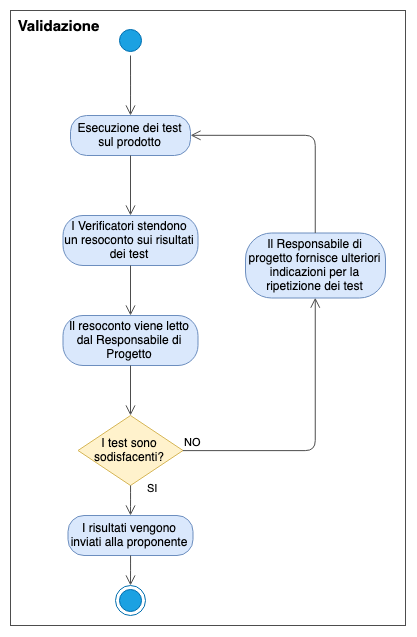
\includegraphics[scale=0.7]{./images/Validazione.png}
	\end{center}
\end{figure}
